\phantomsection
\section*{Chapter 10}
\addcontentsline{toc}{section}{Chapter 10}

\subsection*{10.2}

\begin{figure}[H]
  \centering
  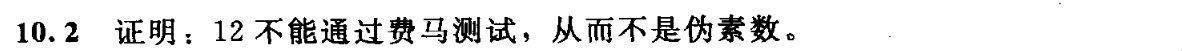
\includegraphics[width=0.8\textwidth]{chapters/imgs/hw_10_2.png}
  \caption{}
  \label{fig:hw_10_2}
\end{figure}

\subsection*{10.4}

\begin{figure}[H]
  \centering
  
\includegraphics[width=0.8\textwidth]{chapters/imgs/hw_10_4.png}
  \caption{}
  \label{fig:hw_10_4}
\end{figure}

\subsection*{10.7}

\begin{figure}[H]
  \centering
  
\includegraphics[width=0.8\textwidth]{chapters/imgs/hw_10_7.png}
  \caption{}
  \label{fig:hw_10_7}
\end{figure}

\subsection*{10.8}

\begin{figure}[H]
  \centering
  
\includegraphics[width=0.8\textwidth]{chapters/imgs/hw_10_8.png}
  \caption{}
  \label{fig:hw_10_8}
\end{figure}

\subsection*{10.10}

\begin{figure}[H]
  \centering
  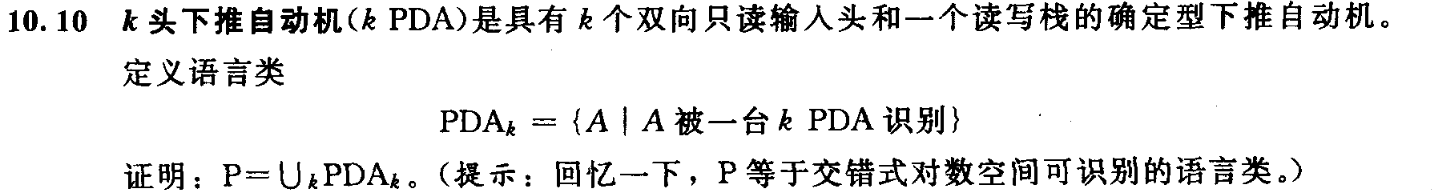
\includegraphics[width=0.8\textwidth]{chapters/imgs/hw_10_10.png}
  \caption{}
  \label{fig:hw_10_10}
\end{figure}

\subsection*{10.13}

\begin{figure}[H]
  \centering
  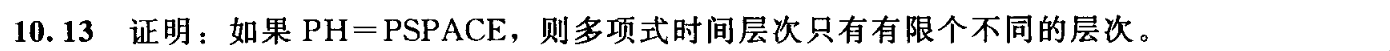
\includegraphics[width=0.8\textwidth]{chapters/imgs/hw_10_13.png}
  \caption{}
  \label{fig:hw_10_13}
\end{figure}

\subsection*{10.19}

\begin{figure}[H]
  \centering
  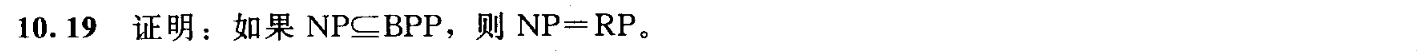
\includegraphics[width=0.8\textwidth]{chapters/imgs/hw_10_19.png}
  \caption{}
  \label{fig:hw_10_19}
\end{figure}

\clearpage
